\documentclass[12pt,a4paper,oneside]{report}

\usepackage{graphicx}
\usepackage{marginnote}
%\usepackage[inner=2cm, outer=2cm]{geometry}
\usepackage[verbose, a4paper, tmargin=2cm, bmargin=2cm, lmargin=2cm, rmargin=2cm, headheight=1.3cm, headsep=1cm]{geometry}
\usepackage{lscape}
%\usepackage[table]{xcolor}
\usepackage{todonotes}
%\usepackage{menukeys}
%\usepackage{listings}
%\usepackage{pdflscape}
%\usepackage{glossaries}
%\usepackage{wrapfig}
%\usepackage{float}
\usepackage{lscape}
%\usepackage{color}

\usepackage{csquotes}
\usepackage[style=numeric, backend=bibtex]{biblatex}
\addbibresource{specification_bibliography}
\defbibheading{secbib}[\bibname]{%
  \section*{#1}%
  \markboth{#1}{#1}}
%\bibliography{specification_bibliography}

% \bibliographystyle{unsrt}

\usepackage{url} 
\usepackage{hyperref}
%\usepackage{natbib}

% ------%

% Code stuff

% ------

\patchcmd{\thebibliography}{\chapter*}{\section*}{}{}

\begin{document}

% ----------------------------------------

\begin{titlepage}

\newcommand{\HRule}{\rule{\linewidth}{0.5mm}} % Defines a new command for the horizontal lines, change thickness here

\center % Center everything on the page
 
%----------------------------------------------------------------------------------------
%	HEADING SECTIONS
%----------------------------------------------------------------------------------------

% University Logo

\includegraphics[width=7cm]{images/uol.png}

%\vfill
%\vfill

\textsc{\LARGE University of Liverpool}\\[1.5cm] % Name of your university/college
\textsc{\large Computer Science with a Year in Industry BSc (Hons)}\\[0.5cm] % Major heading such as course name
\textsc{\large G403}\\[0.5cm] % Minor heading such as course title

%----------------------------------------------------------------------------------------
%	TITLE SECTION
%----------------------------------------------------------------------------------------

\HRule \\[0.4cm]
{ \huge \bfseries COMP390 Honours Year Computer Science Project \\[0.5cm]
Project Specification}\\
[0.4cm] % Title of your document
\HRule \\[1.5cm]
 
%----------------------------------------------------------------------------------------
%	AUTHOR SECTION
%----------------------------------------------------------------------------------------

\begin{minipage}{0.4\textwidth}
\begin{flushleft} \large
\emph{Author:}\\
N Aishah \textsc{B M Senin} \\ (200912462) % Your name
\end{flushleft}
\end{minipage}
~
\begin{minipage}{0.4\textwidth}
\begin{flushright} \large
\emph{Project Advisor:} \\
Dr Prudence \textsc{Wong} % Supervisor's Name
\end{flushright}
\end{minipage}\\[2cm]

% If you don't want a supervisor, uncomment the two lines below and remove the section above
%\Large \emph{Author:}\\
%John \textsc{Smith}\\[3cm] % Your name

%----------------------------------------------------------------------------------------
%	DATE SECTION
%----------------------------------------------------------------------------------------

%{\today}\\[3cm] 
{\large \today}\\[3cm] % Date, change the \today to a set date if you want to be precise

%----------------------------------------------------------------------------------------
%	LOGO SECTION
%----------------------------------------------------------------------------------------

%\includegraphics{Logo}\\[1cm] % Include a department/university logo - this will require the graphicx package
 
%----------------------------------------------------------------------------------------

\vfill % Fill the rest of the page with whitespace

\end{titlepage}

% ----------------------------------------
\section*{Project Description}

% \subsection{What is this project about?}
This project primarily focuses on the animation of different types of commonly used algorithms, for the benefit of users to further understand in depth how algorithms work. However, the scope of this project will only concentrate on algorithmic paradigms, which includes algorithms like \textit{divide and conquer}, \textit{greedy algorithms}, and \textit{dynamic programming}.

Learning what algorithms are and how they work is essential for students who are studying computer science. Since this project is meant to be educational, the target audience of the software will be students studying Computer Science or at least have an interest on how computer programs are made efficient. 

The aim for this project is to allow students to achieve a greater understanding in algorithmic paradigms, by providing an animated explanation in a step by step basis. This is to convey the granulated structure of the algorithms, which allows them to speculate the steps by breaking the complicated algorithm down into smaller parts. This shows the essential pieces of the puzzle that makes the algorithm function as a whole. The program is to allow a play, pause, ``backtrack'', forward and stop functionality, that enables the user to control the animation. I believe that this feature will assist the users to assess the animation at their own pace for a greater learning experience. As for a more comprehensive learning experience, the program is to be flexible by allowing students to input their own values into the program. It will which then use those values to work accordingly to the type of algorithmic method selected. Of course, it would also be a beneficial outcome if this project enables the students to understand different methods of algorithms. This will provide a better perspective and possibly pique their interest on the topic.

\section*{Statement of Deliverables} 
The design documentation, which will be one of the essential documentations, will consist of the architecture of the software, the design of the user interfaces and animations, along with their descriptions of the system features. 

A user documentation on the other hand is written to assist the users on the general use of the software. This documentation will include a user guide and a reference manual, which will be written to explain comprehensively on each feature of the program. There will also be guides for installation (plus uninstallation), and other FAQs pertaining to the program. 

A desirable documentation to have would be one that provides comprehensive information of the algorithms that are available in the program. This documentation will also include the whole script that will be used in the program, describing the steps of each algorithm. Then alongside each animation when played will provide the user a readable content about the algorithms, if the user ever wishes to be more informed about it.

% - anticipated software
For the general outlook of the program, it will list different types of algorithms belonging to the three main approaches to the \textit{algorithmic paradigms}, and other algorithms such as sorting, and binary search trees. Each of these algorithms will have an animated feature, which animates the workings of the algorithm according to what has been selected. When the user selects an algorithm, they will then have an option to put his own input in, or to generate a random value, as its size determines how the animation will be carried out. The user can also interact with the animation by making use of the control buttons, that pauses, plays, ``backtracks'', and stops the animation. During each step of the animation, there will be a short description (or known as the script), about the algorithm's time complexity and description, in either natural language or mathematical, that describes the process of the algorithm.

% - anticipated experiments
The experiments expected in this project revolve around the performance of the system itself. For example, the experiment is to find out the reaction and the feasibility of the animation when a large input is given. Deriving from the conclusion of the experiment, I am to depict the maximum amount of values or set of values that are feasible for the system to handle. 
Another type of experiment would be observing different approaches when solving an algorithmic method, and deduce if the results still produces the same correct result.

% - methods for evaluation of the work
In order to evaluate the quality of the program, I am planning to write the list of criteria the program needs to achieve, such as its usability, user-friendliness, and understandability \nocite{jackson_software_2014}. During the evaluation, I will use the program and conduct the evaluation by writing down comments on the list, whether it is good or needs improvement. If a part of the program does not qualify the criteria, I would then look into redesigning the section accordingly.

\section*{Conduct of the Project and Plan}

% --- Preparation ---
% - Background research
Other than understanding the fundamental workings of the algorithms, there are other aspects of the project that is required of me to conduct a intensive study on. Since I will be implementing my program on a WPF application, I will need to understand its features that are specifically applicable for my project. For instance, it needs to have the necessary user control features and is capable of handling 2D animations. 

WPF applications also uses a specific architectural pattern called the \textit{Model View ViewModel} or \textit{MVVM} \nocite{_mvvm_2012}. It is crucial to be informed of how different parts of the program, the Model, View, and ViewModel works together to function as a whole. It is also important to understand the essence of MVVM as it will greatly depict the overall design and functionality of the program. Last but not least, since I have no experience in writing programs on animations, I might need to research on how to create animations with the use of Microsoft Blend, the IDE that I will be using for the animating aspect of the project \cite{tandon_simple_2007}. From there, I will need to find out the ways on how to \textit{program} my animations, in order to fit the functionality of the algorithm I will be animating.

% --- Design stage ---
Some crucial design documentations include the requirements specification, that will list the functional and non-functional requirements, and the use case diagrams to map out the possible actions between the user (student) and the program. I will also add flowcharts into the design documentation to show a graphical representation of the possible ways the user can interact with the program. Along with them, there will be drawings of what is expected of the graphical user interface, with descriptions on each feature or user control found in the UI. Finally, there will be a section of the design documentation specifically for the animated feature, that includes the designs of the animations. These will be presented in drawings and visualisations of how the animations will be carried out on the program.

% --- Implementation stage ---
% Hardware and software used
As for the implementation stage, the software I will use for the development of the business logic of the WPF application is \textit{Visual Studios 2015 Community Edition}, with C\# as the primary language \cite{_windows_2015}. For the graphical user interface and animations of the algorithms, I will be using \textit{Visual Studios Blend 2015} that uses XAML as a markup language for the GUI \cite{_designing_2015}. The project which will be running on a WPF application, will comfortably run on any Microsoft operating system from Windows 7 onwards.

There will be different stages of testing, both during the implementation and in the testing phase. First of all, I plan to delegate my tasks by breaking my program into units. Once a unit is completed, I will conduct unit testing on it (that is isolated from others \cite{_unit_2003}), and ensure that its code is working as intended. Integration testing, which is an extension of unit testing \cite{_integration_2003}, will be conducted once the interrelated units are completed. Finally, once all the units are being integrated and tested, I will then move on to validation testing which is to test that the program has met all the specifications and fulfilled its intended purpose.

\section*{Risk assessment}
The animation is one of the aspects of this project that holds the highest risk, mainly because I have no experience in doing programmable animations before. Due to this, I also need to ensure that the animation shows a true representation of the algorithmic methods. If an animation is done wrong, there is a possible chance that I may need to redesign and code it again, which can potentially cost a great deal of time. To minimise this risk, I plan to watch various \textit{YouTube} videos of the algorithms, and look at websites that shows animated algorithms, to get better idea of their concepts. On the bright side, with these possible difficulties, I am certain that will acquire new skills and experiences during the course of this project. Such as technical skills like building the software from the ground up, and creating a WPF application that has animated features; to soft skills, such as time management, project management, and problem solving. In other words, this project will definitely be a challenge worth pursuing.
% risk assessment
% major challenges in carrying out the project
% new skills acquired, and how these will be acquired
\printbibliography[heading=secbib]

\begin{landscape}
\begin{figure}[H]
\centering
\hspace*{0cm}
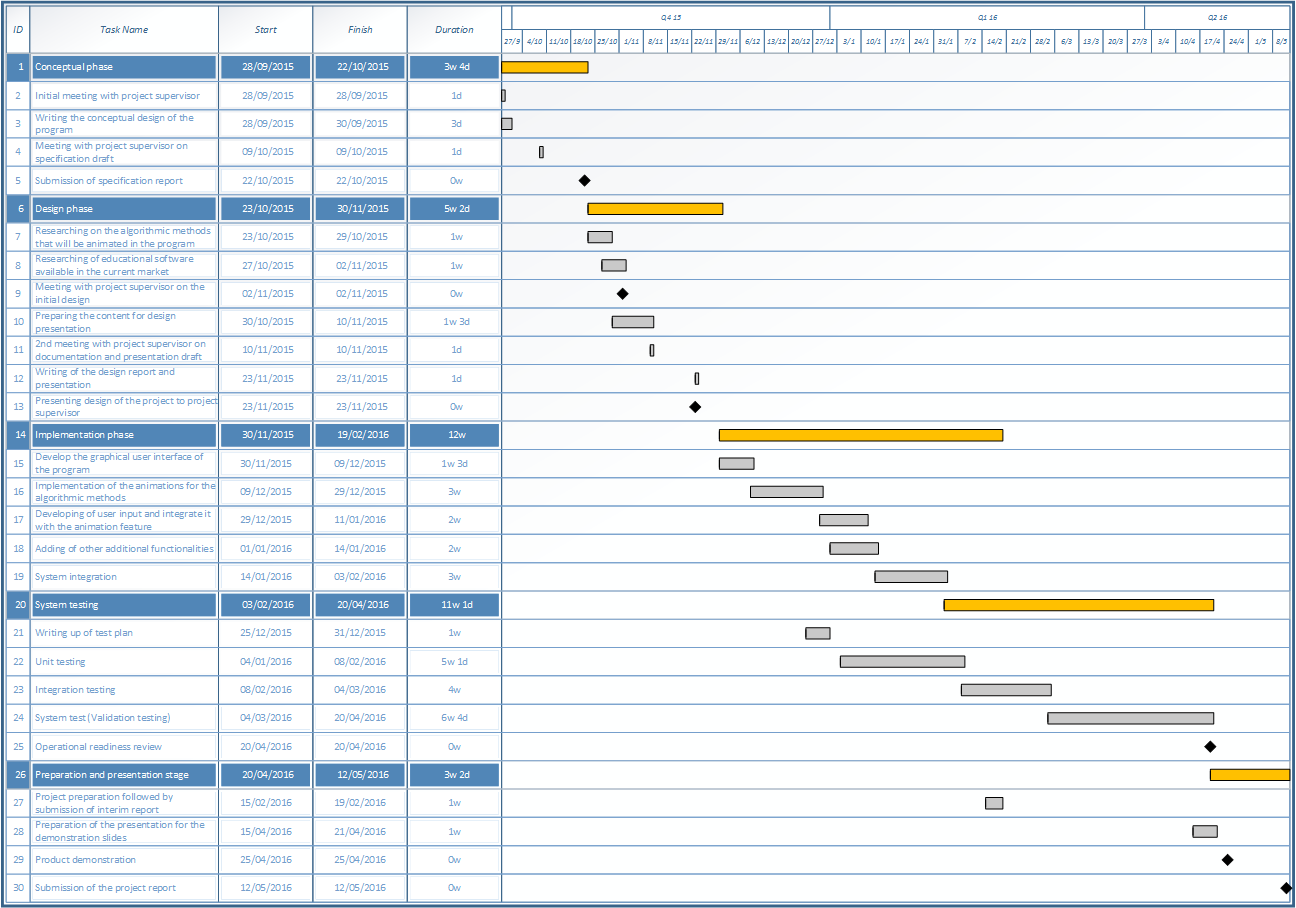
\includegraphics[scale=0.77]{images/specification_ganttChart.png}
\end{figure}
\end{landscape}

%\todototoc
%\listoftodos

\end{document}